% !TEX program = lualatex
\documentclass{matthijs}
\graphicspath{{../assets/}{./docs/assets/}{./docs/technical-design/}}

\begin{filecontents*}[overwrite]{\jobname.xmpdata}
\Title{Technical Design}
\Subject{Implementation description of the lane detection system}
\Author{Matthijs Bakker}
\Language{en-US}
\Keywords{technical\sep design}
\end{filecontents*}

% BEGIN preamble.tex

% Style for first and last page
\usepackage{wallpaper}
\usepackage{color}
\definecolor{arobsblue}{HTML}{0e335c}

% Versioning plugin that retrieves data from the git repo dir
% Needs the "gitInfoHead" file to be generated, make sure
% that the shim script or the git hook is enabled
\usepackage[maxdepth=2]{gitinfo2}

% Use biblatex with biber backend for bibliography
\usepackage{csquotes}
\usepackage[style=ieee]{biblatex}
\renewcommand*{\mkbibacro}[1]{#1}
\setcounter{biburllcpenalty}{7000}
\setcounter{biburlucpenalty}{8000}

% This lets the text look really juicy
\usepackage{microtype}
\usepackage{extdash}

% A column for right-aligned autowrap text
\newcolumntype{R}{>{\arraybackslash}m{10cm}}

% PDF-A
\usepackage{colorprofiles}
\usepackage[a-3b]{pdfx}
\hypersetup{
	bookmarks=true,
	unicode=false,
	pdftoolbar=true,
	pdfmenubar=true,
	colorlinks=true,
	linkcolor=black,
	citecolor=black,
	filecolor=black,
	urlcolor=black
}
%\hypersetup{
%	colorlinks=true,
%	linkcolor=gray,
%	urlcolor=gray,
%	citecolor=gray
%}

% END preamble.tex


\usepackage{titlepage}
\usepackage[title,titletoc]{appendix}

% Load bibliography file
\addbibresource{td.bib}

% Use tikz for drawings
\usepackage{tikz}
\usepackage{tikzscale}
\usepackage{tikz-uml}
\usetikzlibrary{positioning, arrows.meta}
\usepackage{adjustbox}
\usepackage{pgfplots}

% Not quite ConTeXt tables but good enough
\usepackage{colortbl}
\usepackage{multirow}

% IEC/ISO units
\usepackage{amsmath}
\usepackage{siunitx}
\sisetup{detect-all}
\sisetup{output-decimal-marker = {,}}
\DeclareSIUnit{\bit}{b}

\begin{document}

	% Set language to English
	\taal{en}

	\maketitlepage{Technical Design}{0.1}
	\pagenumbering{arabic}
	\thispagestyle{empty}

	\begin{inhoudspagina}

		\clearpage

		%\begin{table}[!ht]
			\begin{tabular*}{\textwidth}{l @{\extracolsep{\fill}} R}
				\toprule

				\textbf{Abbreviation} & \textbf{Definition} \\
				\midrule

				ADAS & Advanced Driver-Assistance System \tabularnewline
				ASIC & A non-reconfigurable digital circuit \tabularnewline
				AXIS & AXI Stream; a bus protocol for data streaming interfaces \tabularnewline
				CLB & Configurable Logic Block; the basic physical component of an FPGA fabric that can contain LUTs, FFs and multiplexers. \tabularnewline
				DMA & Direct Memory Access; a way of reading from / writing to memory without utilizing a processor \tabularnewline
				FPGA & Field Programmable Gate Array; a customizable logic circuit \tabularnewline
				Hard-core processor & A dedicated processor as an ASIC \tabularnewline
				HLS & High Level Synthesis; a technique for synthesizing high level computer code to RTL \tabularnewline
				IPI & Vivado IP Integrator; a tool for integrating IP Cores into block designs \tabularnewline
				IP Core & A pre-made digital logic design \tabularnewline
				MPSoC & Multi-Processor SoC; a SoC with multiple physical processing cores; just a marketing term someone at Xilinx made up \tabularnewline
				PL & Programmable Logic; digital logic that can be reconfigured \tabularnewline
				PS & Processing System; everything related to hard- or softcore processors on the device \tabularnewline
				RTL & Register Transfer Level code; a way of describing the behavior of digital logic \tabularnewline
				SoC & System on Chip; a combination of PL and a hard-core processor \tabularnewline
				Soft-core processor & A processor which is implemented in programmable logic \tabularnewline
				VDMA & Video DMA; A DMA controller specially constructed to read/write video data \tabularnewline
				VPU & Vision Processing Unit; refer to chapter 2 of the Functional Design \tabularnewline

				\bottomrule
			\end{tabular*}
			%\label{tabel:Abbreviations}
		%\end{table}

		\vspace{3ex}

		\textbf{Note:} the abbrevation \textit{DRAM} is ambiguous and is often mixed up in FPGA literature.
		In some situations it means \textit{Distributed RAM} (the memory that can be instantiated in SLICEM LUTs~\cite{xilinxug474}) and in other situations it means \textit{Dynamic RAM} (the external memory that is implemented on our FPGA board).
		To avoid confusion, I will be using the abbrevation \textit{SDRAM} to reference the Dynamic RAM variant.

	\end{inhoudspagina}

	\pagenumbering{arabic}
	\tolerance=1
	\emergencystretch=\maxdimen
	\hyphenpenalty=10000
	\hbadness=10000

	\begin{hoofdstuk}{Preface}

		This project is centered around the realization of an ADAS subsystem which can detect the position of a vehicle within a lane.
		A camera is positioned on the dashboard facing the road in front of the vehicle.
		The video feed from this camera is analyzed in real-time by a computer vision system called the Vision Processing Unit.
		This system is implemented on a Field Programmable Gate Array to achieve low-latency detection.
		The output data, existing of information about the lane the car currently occupies, is passed on to the Lane Departure Warning System so that the car can make decisions with it.

		\bigskip

		This document pertains to the technical side of the system.
		The main goal of this document is to give insight on the inner workings of the system so that the knowledge is preserved and modifications to the system can be easily made in the future.
		Design choices and the overcoming of bottlenecks are mentioned to give advice for future projects.
		Another goal is to describe how the system is integrated in a vehicle so that technicians can troubleshoot issues with it.
		The target audience for this document is whom want to get hands-on with the system and its internals.

		\bigskip

		A global system overview is given in the first paragraph to provide context to the reader.
		In the following paragraphs, the layers of the system are described starting with the hardware layer and ending with the software layer.
		The hardware paragraph is about the physical hardware components which are used in the project.
		The programmable logic layer is about the register transfer level code and how it is synthesized on the FPGA.
		The processing system layer is about the program that runs on the processor.
		The software layer is about the troubleshooting software that runs on an external system and can be used by mechanics to see the internals of the processing unit.

		\bigskip

		In this document I will name binary quantities according to the binary multiples convention as described in ISO/IEC 60027-2:2019, which uses the SI prefixes.
		I choose to use this standard because it is widely used in the embedded industry.
		E.g. one kilobit (\qty{1}{\kilo\bit}) is 1000 bits and one kibibit (\qty{1}{\kibi\bit}) is 1024 bits.

	\end{hoofdstuk}

	\begin{hoofdstuk}{System Overview}

		The goal of this paragraph is to describe the problem that the product will solve in different layers of complexity.
		Each layer will dissect the problem into more complexity than the previous.
		This approach gives context to readers who might not be familiar with the fine technical concepts and who wish to grasp the knowledge at a higher level.

		\begin{paragraaf}{Problem Domain}

			Although the system is not directly controlled by a user, many external forces influence the working of the system.
			We have to take them into account when developing the system because they may affect which choices we will make in the development process and how we integrate the system in a vehicle.

			\begin{figuur}{Operational Problem Domain}
				\singlespacing
				\includegraphics[width=\textwidth]{problem-domain}
				\onehalfspacing
			\end{figuur}

		\end{paragraaf}

		\begin{paragraaf}{Information Context}

		\end{paragraaf}

		\begin{paragraaf}{Component Definition}

			In order to describe which components make up the total system, I have modeled two SysML block diagrams; a Block Definition Diagram (BDD) and an Internal Block Diagram (IBD).
			The BDD shows the components that the system consists of and the Internal Block Diagram shows the relations and interfaces between these components.
			The BDD can be thought of as a black box view that does not represent the inner workings of the system but rather the specifications of it, while the IBD shows exactly how the system is internally composed.

			\begin{figuur}{The System as a SysML Block Definition Diagram}
				\singlespacing
				%\includegraphics[width=\textwidth]{block-definition-diagram}
				\onehalfspacing
			\end{figuur}

		\end{paragraaf}

		\begin{paragraaf}{Implementation Strategy}

			Before starting with the implementation phase, I had to figure out in which layer which parts of the system would need to be implemented.
			Different parts of the system have different advantages, e.g. hardware has the potential to have low latency and fast execution and software excels in decision making.
			I explored the capabilities of the PYNQ-Z2 development board and discovered that it has an SoC with an Artix-7 85K programmable logic fabric and a dual-core ARM Cortex A9 processor.
			The processor comes pre-programmed with an embedded Linux distribution that includes the PYNQ platform.
			This PYNQ platform consists of an FPGA programming framework and a Jupyter webserver.
			The programming framework can be used to program pre-generated bitstreams that were created using Vivado onto the FPGA.
			The Jupyter webserver allows the developer to create code snippets -- so-called 'notebooks' -- that run on the embedded Linux distribution and interact with the Programmable Logic via AXI interfaces.
			These AXI interfaces are hard-IP that connect PS and PL with user-definable 32-bit wide digital connections.
		
			\vspace{-0.6ex}
			\begin{figuur}{The components used for implementing The System}
				\singlespacing
				\includegraphics{implementation-strategy}
				\onehalfspacing
			\end{figuur}
			\vspace{-0.2ex}

			The important concept to understand is that the images which need to be processed are fetched by the Processing System from the capture source.
			I have done this because the connection of a camera is outside the scope of my project and it will be easier to connect the camera to the embedded Linux system because it already has drivers for it.
			Hardware is good at one job, and one job only: the repetetive task it is designed to do, like video processing.
			The results will be delivered back to the PS because it is easier to do business logic like decision making in software.
			This approach also has the benefit of flexibility: software can be modified more quickly than hardware.


		\end{paragraaf}

	\end{hoofdstuk}

	\begin{hoofdstuk}{Integrated Block Design}

		The block design for the system has been created using the Vivado IP Integrator (IPI) because it is the recommended tool to integrate Xilinx IP like the Zynq Processing System in a digital design~\cite{xilinxug994}.
		The design consists of three important components which are connected by diverse utility components.
		These important components are the Zynq Processing System which connects to the hard-core ARMv9 processors, the AXI DMA interface which exchanges memory between PS/PL, and the VPU Image Processing IP Core which is generated by our High Level Synthesis routine.
		The utility components that 'glue' the system in place consist of Xilinx IP Cores like AXI Interconnects that act like buses, AXI Stream Data Width converters that add/remove padding from the video streams and finally the Processor System Reset which manages the reset signals for the interconnects and peripherals.
		\begin{figuur}{Block Diagram of the System Components}
			
			% "This is a big one and it needs some vspace"
			% -- Sasha Gray, 2022
			\vspace{1cm}
			\centerline{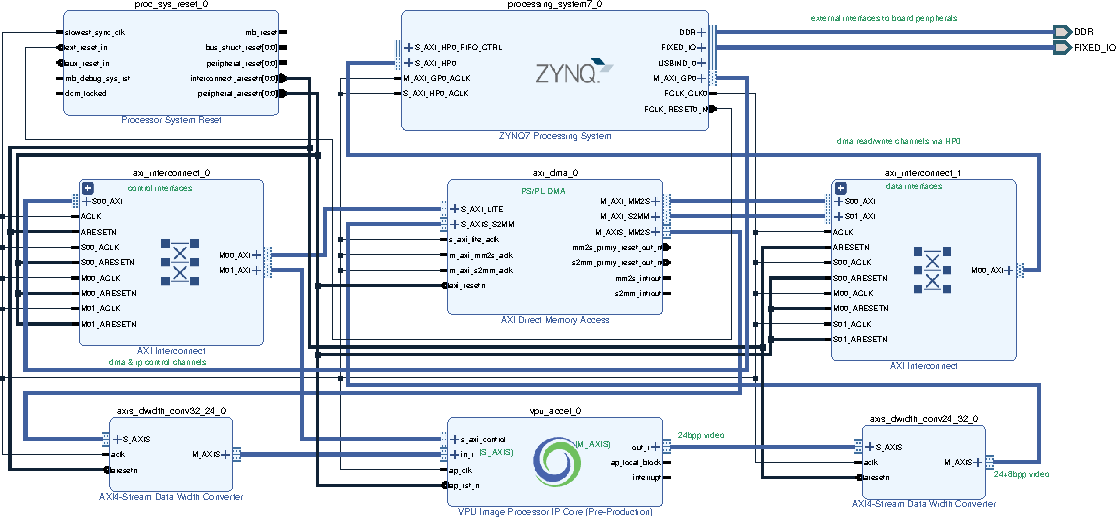
\includegraphics[width=1.2\textwidth]{hw-block-diagram-crop-asset.pdf}}
			\vspace{0.5cm}
			(please see \textit{Appendix}\verwijzingn{paragraaf}{Integrated Block Design Diagram}for a magnified version)

		\end{figuur}

		I've made the decision to only use one global clock net which connects to all components, because I want to prevent components from running off-sync and causing data integrity problems.
		This clock net is derived from the 100MHz system clock.
		As for the reset signal, I had to create different signals for the interconnects and peripherals because those systems cannot be reset at the same time.
		I used the Processor System Reset component to create these reset signals and I connected the interconnect to the reset ports of the interconnects and data width converters.
		The DMA interface and our Image Processor are connected to the peripheral reset net because these need to be reset after the interconnects are up.

		\bigskip

		The Zynq Processing System has multiple types of hard-IP AXI interfaces, including General Purpose~(GP) interfaces and High Performance~(HP) interfaces.
		Although it would be easy to put every component on the HP interface, this is not the proper way to do it.
		For good measure, I have connected the control interfaces of the DMA and the Image Processor to the GP interface using an interconnect.
		Only the DMA interfaces which need to be low-latency are connected to the HP interface.
		This is done using a dedicated interconnect.

		\bigskip

		Vivado automatically assigned addresses for the components which can be used to access them on the HP AXI and the GP AXI-Lite interfaces.
		I have enabled the generation of a Hardware Handoff (HWH) file, which includes these addresses and automatically passes them on to the PYNQ framework.
		This has the benefit of automatically assigning the addresses to the objects in the Jupyter notebooks, and I won't have to work with the raw addresses.
		If the addresses change or get re-assigned, the HWH file will be automatically regenerated by the Vivado Tcl script and the PYNQ references will be automatically updated.

		\begin{figuur}{Memory Mapped Address Assignments on the AXI Buses}

			\centerline{
				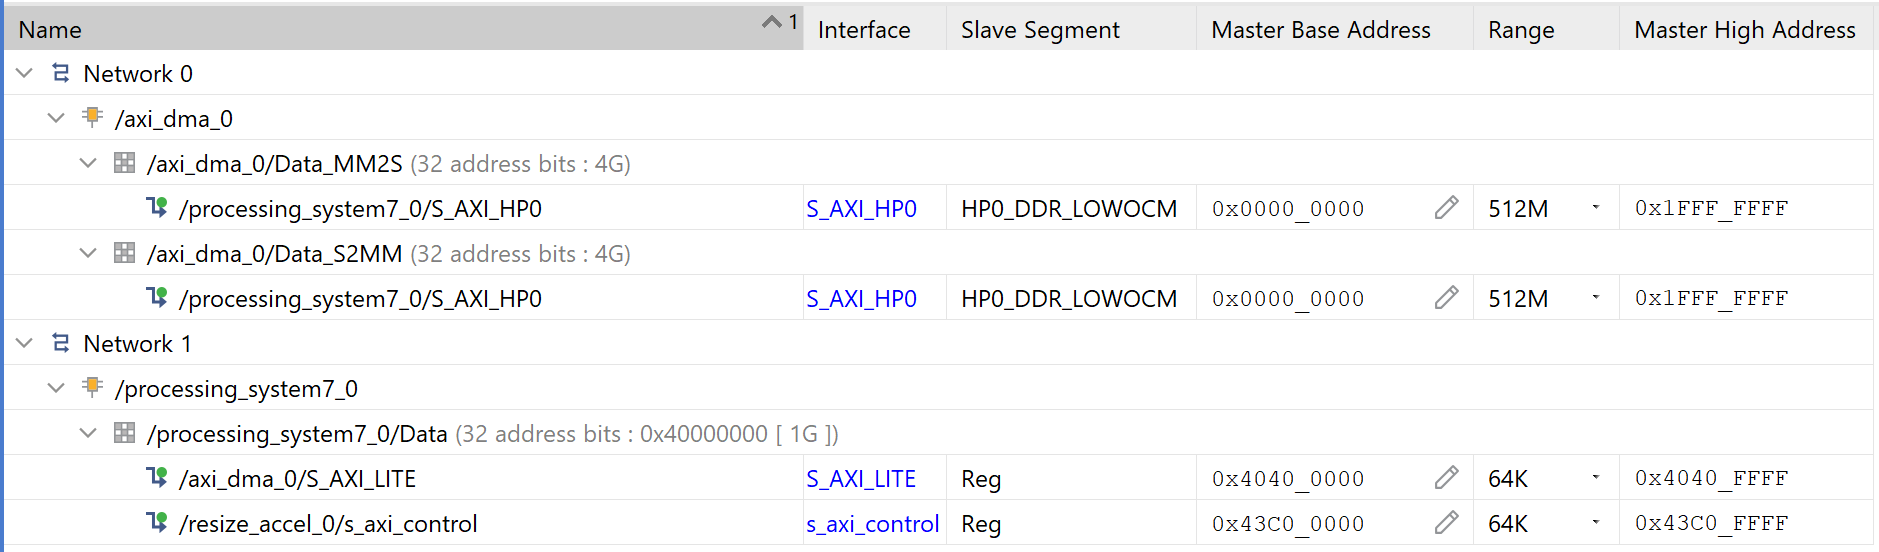
\includegraphics[width=1.1\textwidth, clip, trim=2pt 0 0 2pt]{vivado-bd-address-map-bad-quality.png}
			}

		\end{figuur}
		
		\bigskip

		The DMA is connected to the SDRAM using one of the High Performance AXI ports that comes as hard-IP on the SoC.
		Because the capacity of the SDRAM is half a gibibyte, the range of the memory map has the range to accomodate this.
		It starts at the lowest possible address, 0x0, because the processors expect the system memory to be installed at this location.
		The AXI-HP port has a fixed address size of \qty{32}{\bit}, so this is reflected in the use of the \qty{32}{\bit} addresses for our mapping.
		The DMA is also connected to the Zynq Processing System using an AXI-Lite interface.
		This connection is needed to give control instructions from the software that's running on the PS.

		\bigskip

		Our VPU IP Core is connected to the processing system using AXI-Lite to make the parameters configurable on-the-fly.
		This control interface also provides a way of starting/stopping the video processing function of the core.
		I chose to use an address size of \qty{32}{\bit} to match the size of the hard-IP AXI-GP port that it is connected to.

		\bigskip

		Initially we thought of connecting a camera to the development board to feed the algorithm video data, however, on our new PYNQ board we can simply input images via the framework.
		This change has rendered the camera obsolete, meaning that we don't have to plan I/O pins for it anymore.
		The only pins that are currently used are the hardwired connections and the pre-planned Zynq-PS conections that are retrieved from the board constraints file.
		The package pin planning can be viewed in \verwijzingb{figuur}{FPGA Package Pin Planning}, where orange-marked pins are the pins that are used for the Zynq-PS and connections marked as C or S are hardwired.
		If we wish to use a camera in the future, we have lots of unused pins that could be used to connect it.
		These unused pins are marked with a gray circle on the afforementioned figure.

		\begin{figuur}{FPGA Package Pin Planning}

			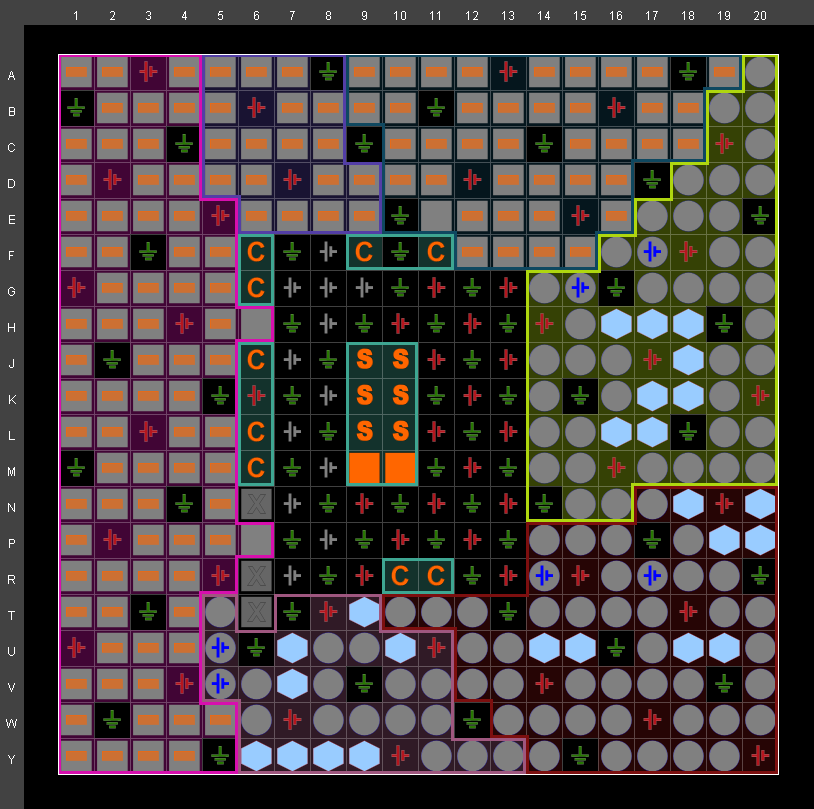
\includegraphics[width=0.8\textwidth]{vivado-synth-package.png}

		\end{figuur}

		Having read up on case studies about high level synthesis, I was worried that we would hit the resource cap because code translation is inherently more inefficient than writing low level code yourself.
		Without creating any timing constraints for the place and route phases, Vivado managed to implement the netlist on the FPGA in an efficient manner.
		It only consumed about 65 percent of the available LUTs and 30 percent of the available FFs while keeping the WNS at \qty{3,2e-11}{\second}, which is 0,3 percent of the clock period. % 0,032 ns :shrug:
		As I talked about in~\verwijzingn{paragraaf}{Memory Configuration}, the BRAM usage is high, but not as high as I expected.
		Due to the proper use of pipelining in the video processing logic, it managed to cram the whole system into only 104 BRAM blocks.
		
		\bigskip

		What I find really interesting is that Vivado has placed the bus infrastructure (AXI interconnects, AXI data width converters, etc) near the Processing System and the VPU IP Core further away from the PS.
		To visualize this in \verwijzingb{figuur}{FPGA Place And Route Floorplan}, I have highlighted with gray color the CLBs that house the bus infrastructure and with yellow color our VPU IP Core.
		This confirms that the place and route phases have been correctly executed and the latency is kept to a minimum.
		It also signals me that I do not need to invest extra time in manually setting timing constraints.

		\vspace{1ex}
		\begin{tabel}{Post-Implementation Utilization Report}{l @{\extracolsep{\fill}} r rr S[table-format=3.1]S[table-format=3.1]}
			\multicolumn{2}{c}{Resource} & \multicolumn{2}{c}{Utilization} & \multicolumn{2}{c}{Utilization \%} \tabularnewline
			\cmidrule{1-2} \cmidrule{3-4} \cmidrule{5-6}
			Type	& Available & \multicolumn{1}{c}{VPU} & \multicolumn{1}{c}{Total}		    & VPU & Total \tabularnewline
			\midrule
			LUT (generic)		& 53200		& 33716 & 36746	& 63.38 & 69.07	\tabularnewline
			LUT (as shift reg)	& 35800		& 276 & 496	& 0.77 & 1.39	\tabularnewline
			LUT (as DRAM)		& 17400		& 48 & 68	& 0.28 & 0.39	\tabularnewline
			FF			& 106400	& 30258 & 34453	& 28.44 & 32.38	\tabularnewline
			DSP			& 220		& 55 & 55	& 25.00 & 25.00	\tabularnewline
			BRAM			& 140		& 99 & 104	& 70.72 & 74.29	\tabularnewline
			BUFG			& 32		& 0 & 1		& 0.00 & 3.13	\tabularnewline

		\end{tabel}

		\begin{figuur}{FPGA Place And Route Floorplan}

			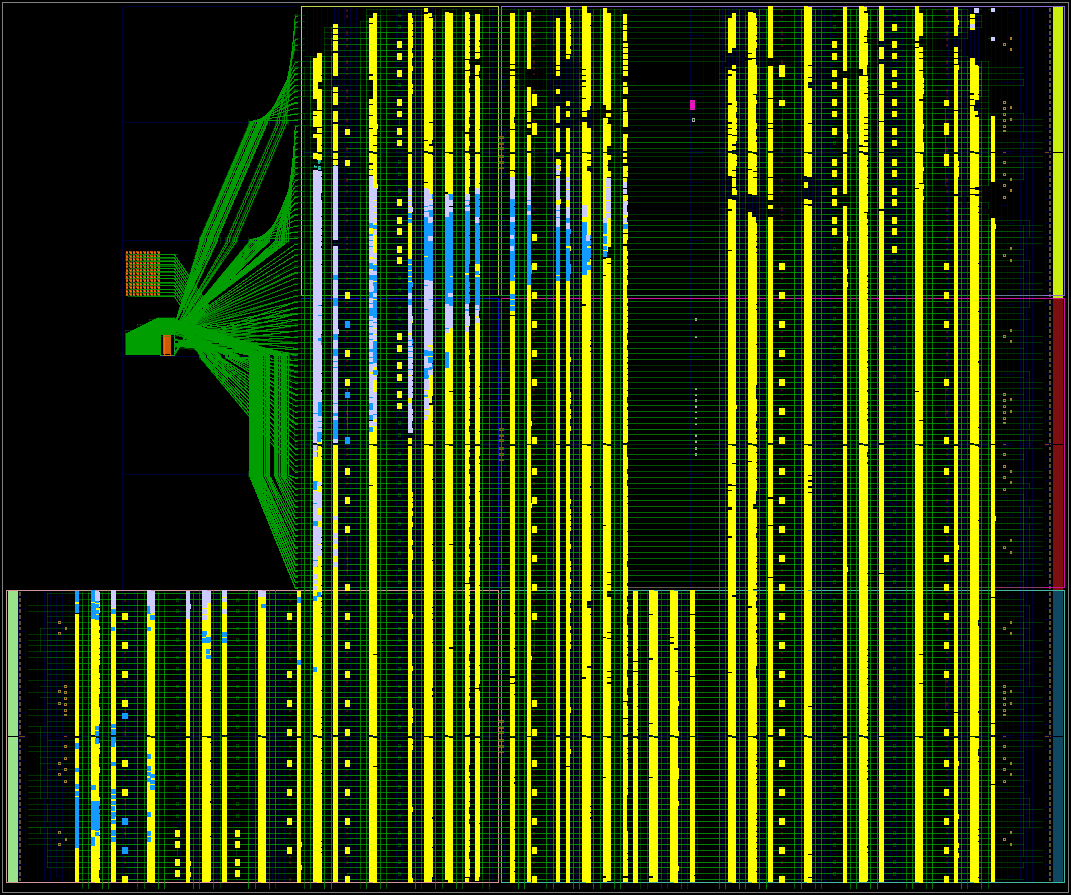
\includegraphics[width=0.8\textwidth]{vivado-impl-placement-full.png}

			\definecolor{floorplanclbwhite}{HTML}{ccccff}
			\definecolor{floorplanclbblue}{HTML}{149bff}
			\definecolor{floorplanclbyellow}{HTML}{ffff00}
			\definecolor{floorplanclbgreen}{HTML}{009e00}

			\vspace{1.5ex}

			\begin{tabular}{rlrl}
				\tikz{\draw[draw=black,fill=floorplanclbwhite] rectangle(1ex, 1ex)} & AXI Bus Infrastructure &
				\tikz{\draw[draw=black,fill=floorplanclbyellow] rectangle(1ex, 1ex)} & VPU IP Core \tabularnewline
				\tikz{\draw[draw=black,fill=floorplanclbblue] rectangle(1ex, 1ex)} & VDMA Controller &
				\tikz{\draw[draw=floorplanclbgreen,line width=0.5mm] (0, 0) -- (1ex, 1ex)} \hspace{-1.325mm} & Connections to PS \tabularnewline
			\end{tabular}

		\end{figuur}

	\end{hoofdstuk}

	\begin{hoofdstuk}{Hardware Layer}

		\begin{paragraaf}{Memory Configuration}

			With the initial development board, the Arty A7-35T, I faced a problem regarding the storage of the video frames.
			It had to do with the limited amount of Block RAM (BRAM) on the FPGA.
			The camera outputs an image of 640 by 480 pixels with a configurable color channel configuration of RGB444, RGB555 or RGB565.
			We prefer to have the highest color depth due to the image processing algorithm working better if there is more input variance.
			The FPGA on the Arty board only had \qty{1800}{\kibi\bit} of BRAM, which was not enough to store a full image frame of the lowest color configuration, as can be seen in \verwijzingb{tabel}{Required space to store images of different sizes}.
			One technique to fit the image into memory is to downscale it, but we would lose information on image features which would have an impact on the quality of detection.

			\begin{tabel}{Required space to store images of different sizes}{l @{\extracolsep{\fill}} r r}
				\emph{Bits per channel (BPC)} & 640$\times$420 px & 320$\times$240 px \tabularnewline
				\midrule
				4+4+4 = 12 b & 3150 Kib & 900 Kib \tabularnewline
				5+5+5 = 15 b & 4500 Kib & 1125 Kib \tabularnewline
				5+6+5 = 16 b & 4800 Kib & 1200 Kib  \tabularnewline
			\end{tabel}
			
			The alternatives places to store an image were the \qty{16}{\mebi\byte} of Quad-SPI flash or the \qty{256}{\mega\byte} DDR3L SDRAM.
			The QSPI flash memory had two downsides: it required controller logic which is only available as an IP Core with a full AXI4 bus, making it difficult to use, and it would have been shared with the MicroBlaze flash sector, so we would have had to make sure not to overwrite those contents.
			The DDR3L SDRAM had one major downside: it required the use of the proprietary Xilinx Memory Interface Generator (MIG) which Digilent does not provide any support for.
			The MIG provides little to no abstraction over the raw DDR3 protocol, making it a challenge of its own to implement it.
			Besides, it is a soft IP, which means that it is delivered in a generic way and the developer has to tailor it to the specific board.
			What makes the SDRAM appealing is its high input clock speed of \qty{166}{\mega\hertz} and the ability to read/write \qty{128}{\bit} of information per cycle.
			This high data throughput would mean that we would not have to worry about speed limitations.
			However, the trade-off between the complexity of implementing the memory interface and the benefits that it would bring would need to be considered.

			\bigskip

			The problems with the memory on the Arty A7 development board as I described above made me question the choice of using this particular board.
			I reevaluated the choice and started exploring other development boards.
			Along the way, I discovered the Zynq-7000 SoC lineup that is officially supported by the Vitis Vision libraries.
			One of the cheapest boards available that has a Zynq-7000 SoC is the TUL PYNQ-Z2.
			The SoC on this development board provides a predefined AXI interconnect between the PL and PS which connects the SDRAM via AXI buses.
			In the PL, this SDRAM can be accessed using a hard IP VDMA controller which provides data over AXI Stream buses.
			These AXI Stream buses can be connected to those on the the Vitis Vision HLS-generated RTL solution.
			Another reason why I chose the PYNQ-Z2 is its larger BRAM capacity; it has \qty{4900}{\kibi\bit} of BRAM.
			However, if using the PYNQ Processing System, this memory will be shared with the processor component, leaving a smaller usable space.
			My final decision is to use the DDR3 SDRAM because it is plentyful on the Z2 board: all \qty{512}{\mega\byte} is available to the developer.

			\bigskip

			The final memory optimization I want to talk about is the use of buffering inside the video processing logic.
			For many image operations (especially those that use convolution, like a simple median filter or the Sobel filter) only a small region of the image is needed for computation at a time.
			Let's think of a simple 3x3 median filter: for each pixel it needs the eight neighbouring pixels to determine the resulting color value.
			To process a row of an image, we would only need to load the pixels of the rows above and below the target row.
			Such a row of pixels is frequently called a "line buffer."
			By using this technique of only loading the pixels that we need to do a regional computation, we do not have to load the entire image into memory and thus we can make way with a smaller amount of memory \cite{hoorick2019convolution}.
			The region that the median kernel operates upon is called a "window."
			In \verwijzingb{figuur}{Line buffering and sliding windows} we can see how the line buffers are used for the image operation.
			
			\begin{figuur}{Line buffering and sliding windows}
				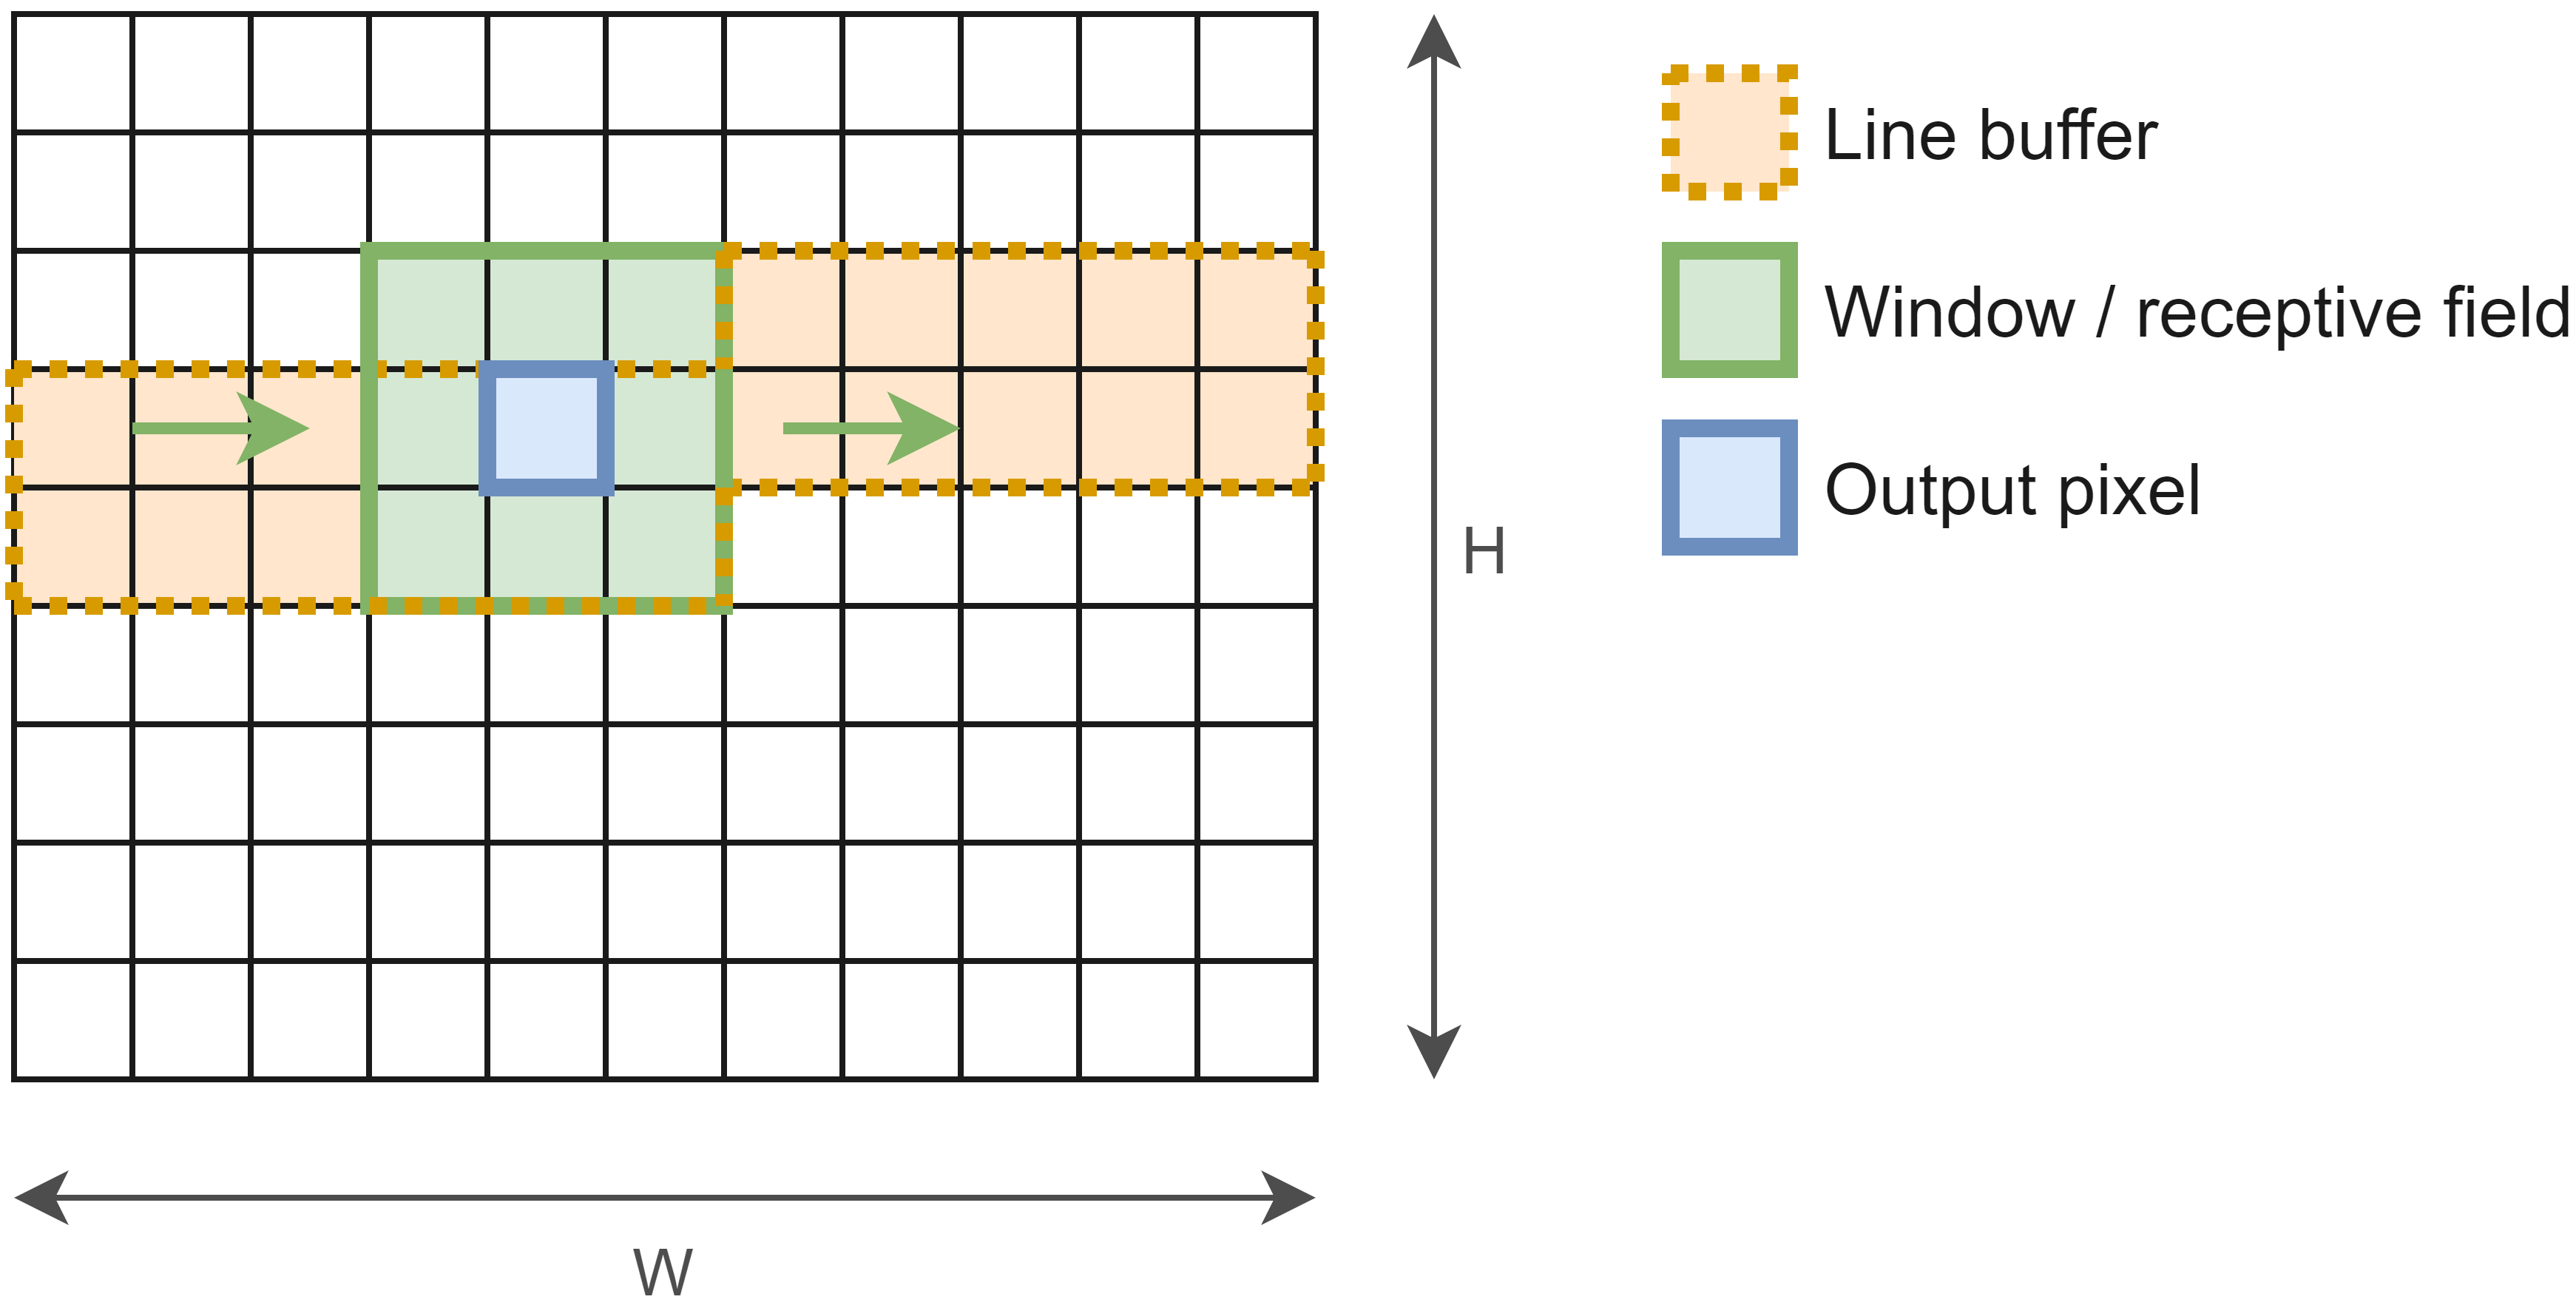
\includegraphics[width=0.8\textwidth]{hoorick2019-convolutions.png}
				\cite{hoorick2019convolution}
			\end{figuur}

			Another advantage of using these line buffers is that we can run the next operation upon the image once the previous operation is done with the lines.
			This is called pipelining, and it enables us to do multiple operations on an image at once with just a small interval between the operations.
			I have used pipelining in the VPU core wherever possible, because it is my goal to reduce image processing latency as much as possible.
			It is my goal to prove that FPGAs are viable for this purpose, so I want to illustrate it with good benchmarks.
			I managed to pipeline all the AXI stream operations, the image color operations, the Gaussian and Sobel filters and the thresholding.
			
			\bigskip

			Unfortunately, I could not apply pipelining to the Hough Transform because this operation needs to have computed all the votes in the accumulator of an image before it can proceed with thinning and sorting of the votes.
			This means that the Hough Transform takes up a lot of memory.
			In fact, I could not even fit the full voting accumulator for the Hough Transform on the FPGA because it used too much BRAM.
			For an image frame of 1280 by 720 pixels, the full accumulator would take up around \qty{6}{\mebi\bit} according to the formula in \verwijzingb{figuur}{Equation for the Hough accumulator size}.
			I needed to lower the theta resolution by two to make the accumulator small enough to fit in the memory.
			The standard full Hough Transform checks 180 angles, but with the reduced $\theta$ resolution it means that we will only check every other angle.
			Consequently, the needed space for the accumulator is halved and fits well within the total of \qty{4,9}{\mebi\bit} available the PYNQ-Z2, leaving room for other components.

			\begin{figuur}{Equation for the Hough accumulator size}

				\vspace{1ex}

				\begin{equation*}
					A_s = \lceil log_e(w) / log_e(2) \rceil \cdot \frac{\theta_{max} - \theta_{min}}{\theta_{res}} \cdot \sqrt{w^2 + h^2}
				\end{equation*}

				\vspace{2ex}

				\textit{Where $w$ and $h$ are the width and height of the input image}

			\end{figuur}

			We can see how much FPGA resources every image processing operation uses by viewing the post-implementation report in Vivado.
			The \textit{utilization} section reports the used resources for every component of the pipeline.

			\begin{tabel}{Resource Utilization per Image Operation}{l @{\extracolsep{\fill}} r r r r}
				\textit{Operation} & BRAM  ($\times$ \qty{18}{\kibi\bit})	& DRAM ($\times$ \qty{64}{\bit})	& DSP	& Generic LUTs	\tabularnewline
				\midrule
				BGR to HSV	& 	& 	& 6	& 391		\tabularnewline
				HSV Threshold	& 6	& 16	& 	& 87		\tabularnewline
				Gaussian Blur	& 5	& 32	& 39	& 3483	 	\tabularnewline
				Sobel Filter	& 3	& 	& 	& 410		\tabularnewline
				Sobel Threshold	& 	& 	& 	& 75		\tabularnewline
				Hough Transform	& 184	& 	& 7	& 27838		\tabularnewline
				Float to Fixed	& 	& 	& 3	& 457		\tabularnewline

			\end{tabel}

			I did not specifically include the shift registers in \verwijzingb{tabel}{Resource Utilization per Image Operation} because those can be implemented in non-SLICEM LUTs as well, of which there are plenty.
			We can confirm from this report that the Hough Transform is very memory intensive.
			The storage of the vote accumulator used a total of 92 RAMB36E1 blocks, resulting in a total of \qty{3312}{\kibi\bit} being instantiated for the Hough Transform alone.
			This is almost 70 percent of the total BRAM available on the FPGA.
			Convolution-based image operations like the Gaussian Blur and the Sobel Operator were implemented with very little memory required.
			This is because of the line buffers and aggressive pipelining.
			They hand over data to the next function after processing only a few lines, and thus not requiring much storage.

		\end{paragraaf}

		\clearpage

		\begin{paragraaf}{Communication Workflow between the PS and the PL}
			
			What makes the Zynq SoC appealing is that is has a hard-IP memory controller that is directly connected to the SDRAM.
			Therefore, the developer does not need to implement the DDR3 memory interface themselves.
			I used this benefit to my advantage; my strategy is to place the images into memory using the CPU and then access them using VDMA in the digital logic.
			This leaves the BRAM/DRAM available for the image processing logic.
			The VDMA IP Cores with the driving logic for the memory interface are supplied by Xilinx, requiring little work on my part to fetch the images in PL.

			\vspace{-0.6ex}
			\begin{figuur}{Classic hardware co-processing compared to FPGA co-processing}
				\singlespacing
				\includegraphics{coprocessing}
				\onehalfspacing
				\vspace{-2ex}
			\end{figuur}
			\vspace{-0.2ex}

			The way the memory is used on the Zynq-7000 with VDMA reminds me of using the OpenGL and Vulkan graphics APIs.
			With OpenGL, you would allocate 'textures' and other data the GPU needs in the host memory and then pass a reference to the data to the shader program that would run on the GPU.
			With Vulkan, this process would be a bit more detailed and you would have to manually specify how you would stream the textures/data to the VRAM before being able to access this data from the shader.
			And now, with Zynq, we would allocate the data in host memory, stream the data to the BRAM/DRAM using the VDMA and then run the kernel by setting the register.
			After the data is processed, the VDMA feeds the results back into the buffer in host memory that we allocated.
			I did a lot of graphics programming a few years back, so I was able to see the similarities between these practices and adapt them to FPGA co-processing.
			
			\bigskip

			The transaction between software and hardware starts by allocating memory in the host's SDRAM by using the Xilinx Runtime (XRT) framework.
			This space will be accessible by the Programmable Logic via the VDMA.
			First, we copy the image into this memory space in the driver software.
			Subsequently, we send the address pointer to the VDMA IP Core in the Programmable Logic over the general-purpose AXI-Lite bus so that it knows where the image is located.
			This VDMA component is connected to our VPU IP Core using an AXI Stream, and the VDMA will provide the image data over this stream as soon as it is available.
			Then, we send a command to the VPU IP Core over it's AXI-Lite interface that it can start processing the data.

			\vspace{-0.6ex}
			\begin{figuur}{Communication between Host and Accelerator in Co-processing Methodology}
				\singlespacing
				\begin{adjustbox}{width=\textwidth,center}
					\includegraphics{coproseq}
				\end{adjustbox}
				\onehalfspacing
				\vspace{-2ex}
			\end{figuur}
			\vspace{-0.2ex}

			Once the VPU IP Core is done with processing the data, it pulls the TLAST wire on the output AXIS interface high.
			This rising edge signals the VDMA that the data transfer is complete and that the receive channel should close.
			The output image data now resides at the output buffer location in the SDRAM and can be retrieved by the driver software running on the Processing System.
			A more detailed illustration of this process can be seen in \verwijzingb{figuur}{Communication between Host and Accelerator in Co-processing Methodology}.

		\end{paragraaf}

		\textbf{[todo:]}

	\end{hoofdstuk}

	\begin{hoofdstuk}{Programmable Logic Layer}

		\begin{paragraaf}{Lane Detection IP}

			% ----- Introductie; wat is HLS en Vitis Vision?
			I chose to implement the image processing stages using High Level Synthesis because Xilinx provides a well-designed OpenCV port that is tested and formally proven.
			This port was formerly called xfOpenCV prior to it being integrated into the Vitis standard libraries and renamed to Vitis Vision.
			It is a clean-room implementation of OpenCV functions that includes instruction pragmas which tell the compiler how certain code should be synthesized to RTL.
			These pragmas include information on how certain loops should be unrolled and how variables can be synthesized to registers.
			The developer can write C++ code which specifies which AXI interfaces have to be created and which vision functions have to be applied.
			This code can be simulated on the developer's system using the official OpenCV library to verify the working of the code.
			Once verified, the code can be synthesized to HDL and can be co-simulated to verify that the automatically generated HDL performs exactly like the original code.
			Finally, Vivado can synthesize the HDL to a netlist and implement it into an IP Core, which can be used in other projects.
			

			\bigskip

			% ----- Hoe heb ik de vision libs gebruikt?
			\textbf{[todo: leg uit, een AXI stream voor input en voor output]}

			\bigskip

			\textbf{[todo: plaatje van regio dichtbij de VPU core]}

			% ----- Hoe heb ik de IP Core geintegreerd in het systeem?
			I incorporated this IP Core into the block design using the IPI and connected it to the DMA component with Xilinx AXI Stream Data Width Converters on the input and output streams.
			These converters are necessary because the AXI HP ports are fixed to a \qty{32}{\bit} width.
			The software driver is configured to pad the output stream with zeroes up to this \qty{32}{\bit} width.
			From the software, we send the memory location of a RGB888 video frame that is stored in the SDRAM to the DMA via its AXI-Lite port, which will initiate the transfer via the \qty{32}{\bit} wide bus to the converter, which, in turn, will ignore the padding by only transferring the first \qty{24}{\bit}.
			This step causes the data to become available on the input interface of the VPU core.
			Next, we set the \textit{AP\_START} and \textit{AP\_AUTOSTART} bits of the memory-mapped control register of the VPU core via its AXI-Lite interface.
			This will toggle the VPU core into a mode where it automatically processes the data available on the input stream.
			The start/stop/etc control logic is implemented with the "return" pragma in the VPU code and is generated by Vitis, ensuring that it is correct.
			To express this in FPGA terminology, we can think of 'inference' of this control interface.
			Upon completion of the processing of the entire video frame, the VPU core autonomously writes the resulting data to the output stream.
			The output is a 8-bit-per-pixel grayscale image which helps technicians debug the system, as described in the user stories of the Functional Design.
			Although four pixels would theoretically fit in one data transfer, the output currently only sends one pixel per transfer, resulting in a total output width of eight bits.
			The outbound data width converter adds \qty{24}{\bit} of padding to make up for the AXI-HP port's fixed width.
			Both the input and output stream interfaces have FIFO queues implemented as underlying buffers.
			I did this to deal with the backpressure of the data width converters; the VPU IP core can take multiple clock cycles to read/write to/from the streams, while the AXI infrastructure components always transfer one pixel per clock cycle.

			\textbf{[todo: tabel met memory mapping van de VPU IP core registers]}

			\textbf{[todo:]}

		\end{paragraaf}

		\textbf{[todo:]}

	\end{hoofdstuk}

	\begin{hoofdstuk}{Processing System Layer}

		\textbf{[todo:]}

	\end{hoofdstuk}
	
	\begin{hoofdstuk}{Software Layer}

		\textbf{[todo:]}

	\end{hoofdstuk}

	\begin{hoofdstuk}{Benchmarks}

		The reason of doing the heavy processing in hardware is to gain a speed advantage over software implementations.
		I have set up benchmarks in which I have compared the performance of the test program that I created as part of the research phase to OpenCV and finally to the FPGA implementation.
		Besides processing speed, I will also compare the power draw and efficiency of the different solutions.

		\begin{paragraaf}{Power Efficiency}

			Using hardware cosimulation in Vitis, it is possible to estimate the power draw of the FPGA chip.
			However, these metrics only take into account the FPGA fabric and not the ARM Cortex processor that is also embedded in the Zynq package.
			In Vivado, the power estimation report tool \textit{does} try to take into account the power draw of the processing system.
			This is marked in~\verwijzingb{figuur}{Total SoC Power Estimation}~with the PS7 label.
			However, since it does not know the code that will run on the processor and thus cannot estimate the processor load, it presumes a constant load of 50 percent.
			This is confirmed to be the case in~\verwijzingb{figuur}{CPU Power Estimation}.
			I think it gives more insight to compare only the metrics of the actual video processing logic between solutions because the driver code is unpredictable.
			Therefore, I will only compare the power consumption of the accelerator chips (GPU, FPGA) with each other.

			\vspace{1.5ex}
			\begin{figuur}{Total SoC Power Estimation}
				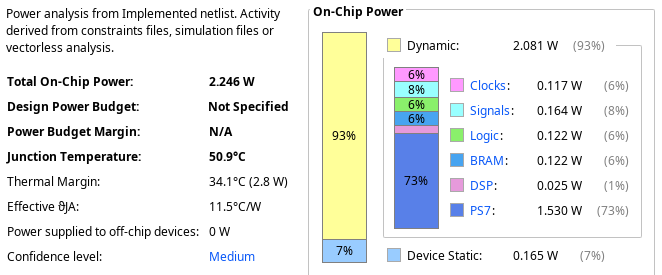
\includegraphics[width=0.85\textwidth]{vivado-power.png}
			\end{figuur}
			\begin{figuur}{CPU Power Estimation}
				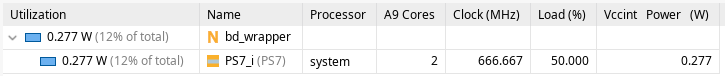
\includegraphics[width=\textwidth]{vivado-power-ps.png}
			\end{figuur}

			To benchmark the power consumption OpenCV reference code from my HLS testbenches, I used the AMD ROCm SMI tools.
			This library could read the power draw as reported by my iGPU.
			Note that my iGPU was not dedicated to the CV code alone; it was also used by other programs like my desktop environment.
			For this reason, the power draw is an estimation and should not be interpreted as being accurate.

		\end{paragraaf}

		\begin{paragraaf}{Execution Speed}

			It is possible to calculate the precise execution speed of the video processing logic by looking at the number of clock cycles needed for the pipelines to finish.
			The time in seconds can be calculated by dividing the number of clock cycles with the system clock speed of \qty{100}{\mega\hertz}.
			However, we have to take into account that, due to pipelining, the top left pixel of an image is transmitted (but also received) earlier than the bottom right pixel.
			The \textit{minimum latency} is the time between the transmission and return of the first pixel.
			The \textit{maximum latency} is the time spent between the transmission of the first pixel and the receiving of the last pixel.
			Thus, the maximum latency is a good metric to use for measuring the processing time of a single frame.
			For the whole video processing pipeline, including writing/reading image data to/from the local memory, the required cycles per operation is 1119344, which translates to \qty{11.19}{\milli\second}.

			\begin{figuur}{Vitis Timing Report for the VPU Logic}
				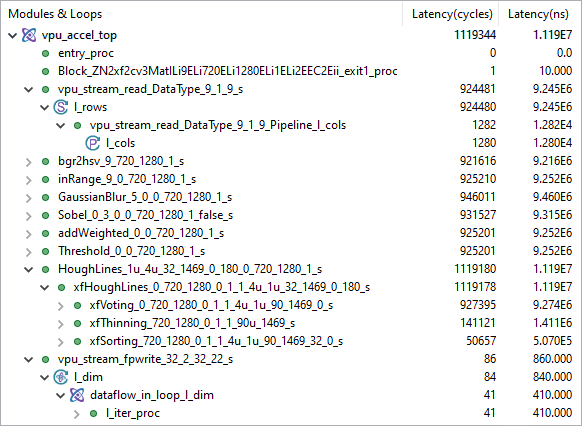
\includegraphics[width=0.75\textwidth]{vitis-timing-bad-quality.png}
			\end{figuur}

			However, we also have to take into account the run time of the driver logic.
			I wrote the simple driver code using the PYNQ framework as it came preinstalled on the development board.
			The PYNQ framework is meant for rapid prototyping and is not meant for high performance situations.
			Instead of writing a barebones low-level application to run directly on the ARM Cortex core, PYNQ offers a Linux-based OS with a Python interpreter that can access the XRT and can interface with the FPGA hardware.
			When measuring the run time of the Python driver code, it took \qty{26.6}{\milli\second} ± \qty{443}{\micro\second} (mean std. dev. over 500 iterations) for the complete handling and processing of an image.
			As this is more than twice the total latency of the image processing alone, I suspect that the framework handles the memory operations inefficiently.
			Nevertheless, the frames per second that the code is able to process is still higher than that of a studio movie, so I'm quite happy with the speed of execution.

			\bigskip

			To measure the reference OpenCV execution speed, I used the \textit{TickMeter} class because it is part of the OpenCV core.
			I figured it would be better to use standardized methods than to roll my own.
			By using the TAPI introduced in OpenCV 3, I only had to make one change to my existing host code to run it on my iGPU: change the \textit{Mat} data type to \textit{UMat}.
			This data type is a generic one that can hold the data in the VRAM behind abstraction.
			I ran the reference programs on my laptop with a Ryzen 5 2500U with integrated graphics.

			\bigskip

			For running the OpenCV reference program, I isolated four CPU cores from the OS scheduler and dedicated them to the program.
			I also measured the performance of the test implementation (aka "Lane Program", I didn't have much inspiration for its name) that I made during the research phase of the project.
			This program is executed on the CPU and is only capable of using a single thread.
			For running the Lane Program, I dedicated one of the isolated cores to it.
			Except for the raw FPGA implementation, for which we can calculate the latency exactly, I ran all tests 500 times and calculated the average run time and standard deviation between run times.

			\bigskip

			\begin{tabel}{Performance comparison per platform}{l @{\extracolsep{\fill}} S[table-format=3.1]S[table-format=3.1]}
				Platform & {Average (ms)} & {Standard Deviation (ms)} \tabularnewline
				\midrule

				FPGA (raw)		& 11.2		& {-} 		\tabularnewline
				FPGA (co-processing)	& 26.6		& 0.443		\tabularnewline
				Reference OpenCV (CPU)	& 72.2		& 1.801		\tabularnewline
				Reference OpenCV (GPU)	& 14.2		& 0.794		\tabularnewline
				Reference Lane Program	& 382.7		& 13.81		\tabularnewline

			\end{tabel}

			\begin{figuur}{Bar chart performance comparison per platform}
				\centerline{
					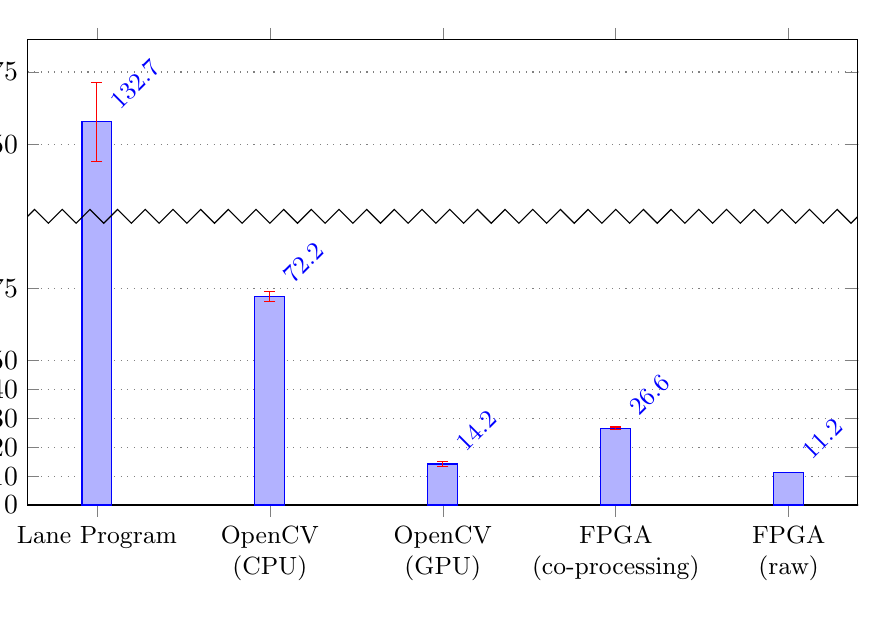
\begin{tikzpicture}[trim axis left, trim axis right]
					\begin{axis}[
						width=\textwidth,
						height=49.5ex,
						ybar,
						ymin=0,
						bar width=2.5ex,
						ylabel={
							milliseconds per execution \\
							\textit{(less is better)}
						},
						ylabel style={
							align=center,
							yshift=1ex
						},
						/tikz/every pin/.style={align=center},
						symbolic x coords={
							Lane Program,
							OpenCV (CPU),
							OpenCV (GPU),
							FPGA (coprocessing),
							FPGA (raw)
						},
						xtick=data,
						ytick=      {0, 10, 20, 30, 40, 50, 75, 125, 150},
						yticklabels={0, 10, 20, 30, 40, 50, 75, 350, 375, 400},
						x tick label style={align=center, font=\small},
						xticklabels={
							FPGA\\(raw),
							FPGA\\(co-processing),
							OpenCV\\(GPU),
							OpenCV\\(CPU),
							Lane Program
						},
						grid style={dotted, gray},
						ymajorgrids=true,
						nodes near coords,
						every node near coord/.append style={
							font=\small,
							align=left,
							rotate=45,
							anchor=south west,
							xshift=1.25ex,
							yshift=-1.5ex
						}
					]
						\addplot+[
							%restrict y to domain=0:100,
							error bars/error bar style={red},
							error bars/.cd, y dir=both, y explicit
						] coordinates {
							(FPGA (raw),		11.2)
							(FPGA (coprocessing),	26.6) +- (0, 0.443)
							(OpenCV (GPU),		14.2) +- (0, 0.794)
							(OpenCV (CPU),		72.2) +- (0, 1.801)
							(Lane Program,		132.7) +- (0, 13.81)
						};
					\coordinate (V) at (axis cs:Lane Program,100);
					\coordinate (H1) at (rel axis cs:0,0);
					\coordinate (H2) at (rel axis cs:1,0);
					\draw[black] decorate [decoration={zigzag}] {(V -| H1) -- (V -| H2)};
					\end{axis}
				\end{tikzpicture}
				}
				\vspace{-1ex}
			\end{figuur}

		\end{paragraaf}

	\end{hoofdstuk}
	
	% Bibliography page
	\begin{hoofdstuk}{References}

		\printbibliography[heading=none]

	\end{hoofdstuk}

	\begin{appendices}
		\begin{hoofdstuk}{Enlarged Figures}
			\begin{paragraaf}{Integrated Block Design Diagram}
				\vspace{0.25cm}
				\centerline{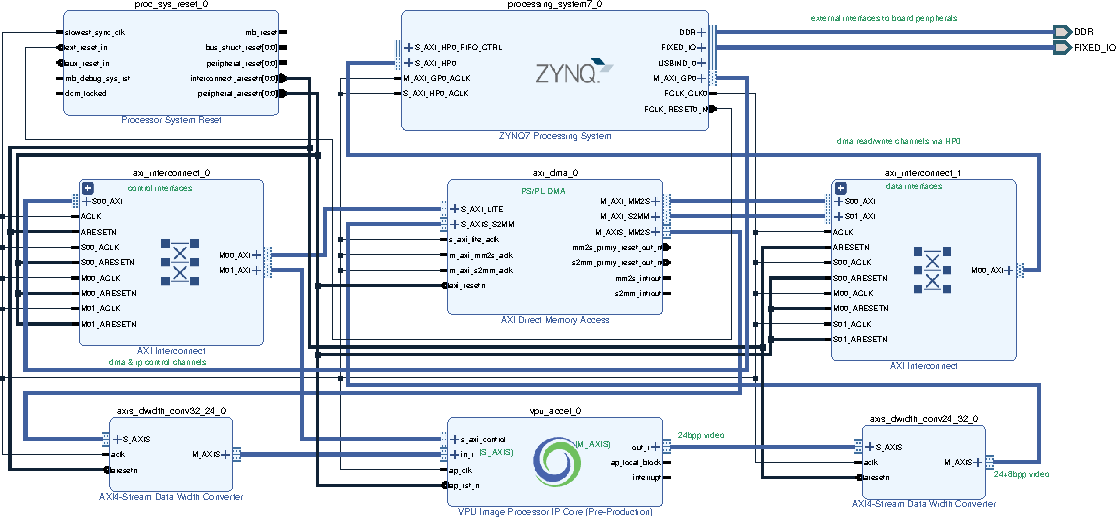
\includegraphics[angle=90, origin=c, clip, trim=9.45cm 0 0 0, width=1.25\textwidth]{hw-block-diagram-crop-asset.pdf}}
				\clearpage
				\centerline{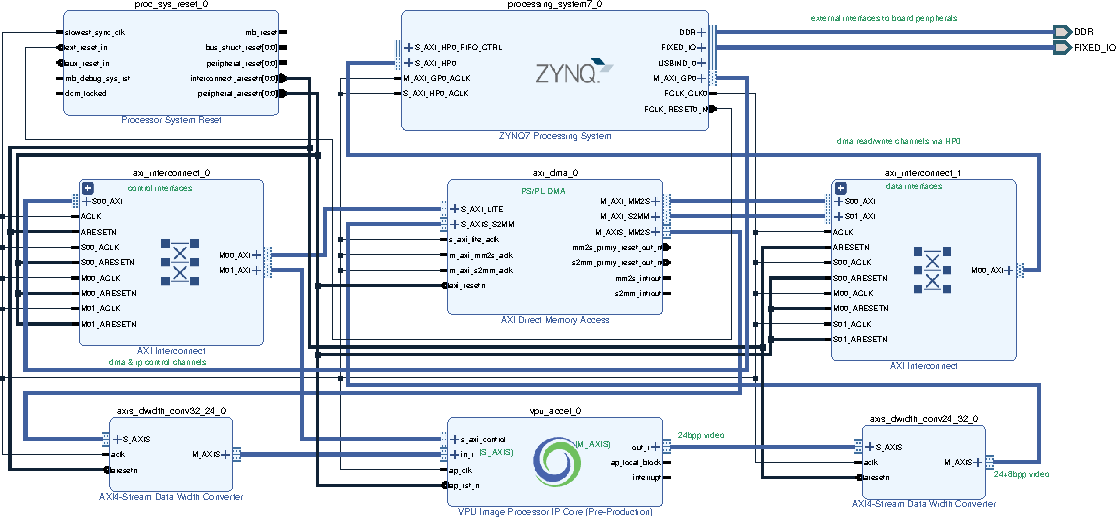
\includegraphics[angle=90, origin=c, clip, trim=0 0 9.45cm 0, width=1.25\textwidth]{hw-block-diagram-crop-asset.pdf}}
			\end{paragraaf}
		\end{hoofdstuk}
	\end{appendices}

	% Empty last page
	\clearpage
	\thispagestyle{empty}
	\addtocounter{page}{-1}
	\ThisULCornerWallPaper{1.005}{asset_bg_last_page.jpg}
	\
	\clearpage

\end{document}
